%%%%%%%%%%%%%%%%%%%%%%%%%%%%%%%%%%%%%%%%%
% Lachaise Assignment
% LaTeX Template
% Version 1.0 (26/6/2018)
%
% This template originates from:
% http://www.LaTeXTemplates.com
%
% Authors:
% Marion Lachaise & François Févotte
% Vel (vel@LaTeXTemplates.com)
%
% License:
% CC BY-NC-SA 3.0 (http://creativecommons.org/licenses/by-nc-sa/3.0/)
% 
%%%%%%%%%%%%%%%%%%%%%%%%%%%%%%%%%%%%%%%%%

%----------------------------------------------------------------------------------------
%	PACKAGES AND OTHER DOCUMENT CONFIGURATIONS
%----------------------------------------------------------------------------------------

\documentclass{article}

%%%%%%%%%%%%%%%%%%%%%%%%%%%%%%%%%%%%%%%%%
% Lachaise Assignment
% Structure Specification File
% Version 1.0 (26/6/2018)
%
% This template originates from:
% http://www.LaTeXTemplates.com
%
% Authors:
% Marion Lachaise & François Févotte
% Vel (vel@LaTeXTemplates.com)
%
% License:
% CC BY-NC-SA 3.0 (http://creativecommons.org/licenses/by-nc-sa/3.0/)
% 
%%%%%%%%%%%%%%%%%%%%%%%%%%%%%%%%%%%%%%%%%

%----------------------------------------------------------------------------------------
%	PACKAGES AND OTHER DOCUMENT CONFIGURATIONS
%----------------------------------------------------------------------------------------

\usepackage{amsmath,amsfonts,stmaryrd,amssymb} % Math packages

\usepackage{enumerate} % Custom item numbers for enumerations

\usepackage[ruled]{algorithm2e} % Algorithms

\usepackage[framemethod=tikz]{mdframed} % Allows defining custom boxed/framed environments

\usepackage{listings} % File listings, with syntax highlighting
\lstset{
	basicstyle=\ttfamily, % Typeset listings in monospace font
}

%----------------------------------------------------------------------------------------
%	DOCUMENT MARGINS
%----------------------------------------------------------------------------------------

\usepackage{geometry} % Required for adjusting page dimensions and margins

\geometry{
	paper=a4paper, % Paper size, change to letterpaper for US letter size
	top=2.5cm, % Top margin
	bottom=3cm, % Bottom margin
	left=2.5cm, % Left margin
	right=2.5cm, % Right margin
	headheight=14pt, % Header height
	footskip=1.5cm, % Space from the bottom margin to the baseline of the footer
	headsep=1.2cm, % Space from the top margin to the baseline of the header
	%showframe, % Uncomment to show how the type block is set on the page
}

%----------------------------------------------------------------------------------------
%	FONTS
%----------------------------------------------------------------------------------------

\usepackage[utf8]{inputenc} % Required for inputting international characters
\usepackage[T1]{fontenc} % Output font encoding for international characters

\usepackage{XCharter} % Use the XCharter fonts

%----------------------------------------------------------------------------------------
%	COMMAND LINE ENVIRONMENT
%----------------------------------------------------------------------------------------

% Usage:
% \begin{commandline}
%	\begin{verbatim}
%		$ ls
%		
%		Applications	Desktop	...
%	\end{verbatim}
% \end{commandline}

\mdfdefinestyle{commandline}{
	leftmargin=10pt,
	rightmargin=10pt,
	innerleftmargin=15pt,
	middlelinecolor=black!50!white,
	middlelinewidth=2pt,
	frametitlerule=false,
	backgroundcolor=black!5!white,
	frametitle={Command Line},
	frametitlefont={\normalfont\sffamily\color{white}\hspace{-1em}},
	frametitlebackgroundcolor=black!50!white,
	nobreak,
}

% Define a custom environment for command-line snapshots
\newenvironment{commandline}{
	\medskip
	\begin{mdframed}[style=commandline]
}{
	\end{mdframed}
	\medskip
}

%----------------------------------------------------------------------------------------
%	FILE CONTENTS ENVIRONMENT
%----------------------------------------------------------------------------------------

% Usage:
% \begin{file}[optional filename, defaults to "File"]
%	File contents, for example, with a listings environment
% \end{file}

\mdfdefinestyle{file}{
	innertopmargin=1.6\baselineskip,
	innerbottommargin=0.8\baselineskip,
	topline=false, bottomline=false,
	leftline=false, rightline=false,
	leftmargin=2cm,
	rightmargin=2cm,
	singleextra={%
		\draw[fill=black!10!white](P)++(0,-1.2em)rectangle(P-|O);
		\node[anchor=north west]
		at(P-|O){\ttfamily\mdfilename};
		%
		\def\l{3em}
		\draw(O-|P)++(-\l,0)--++(\l,\l)--(P)--(P-|O)--(O)--cycle;
		\draw(O-|P)++(-\l,0)--++(0,\l)--++(\l,0);
	},
	nobreak,
}

% Define a custom environment for file contents
\newenvironment{file}[1][File]{ % Set the default filename to "File"
	\medskip
	\newcommand{\mdfilename}{#1}
	\begin{mdframed}[style=file]
}{
	\end{mdframed}
	\medskip
}

%----------------------------------------------------------------------------------------
%	NUMBERED QUESTIONS ENVIRONMENT
%----------------------------------------------------------------------------------------

% Usage:
% \begin{question}[optional title]
%	Question contents
% \end{question}

\mdfdefinestyle{question}{
	innertopmargin=1.2\baselineskip,
	innerbottommargin=0.8\baselineskip,
	roundcorner=5pt,
	nobreak,
	singleextra={%
		\draw(P-|O)node[xshift=1em,anchor=west,fill=white,draw,rounded corners=5pt]{%
		Question \theQuestion\questionTitle};
	},
}

\newcounter{Question} % Stores the current question number that gets iterated with each new question

% Define a custom environment for numbered questions
\newenvironment{question}[1][\unskip]{
	\bigskip
	\stepcounter{Question}
	\newcommand{\questionTitle}{~#1}
	\begin{mdframed}[style=question]
}{
	\end{mdframed}
	\medskip
}

%----------------------------------------------------------------------------------------
%	WARNING TEXT ENVIRONMENT
%----------------------------------------------------------------------------------------

% Usage:
% \begin{warn}[optional title, defaults to "Warning:"]
%	Contents
% \end{warn}

\mdfdefinestyle{warning}{
	topline=false, bottomline=false,
	leftline=false, rightline=false,
	nobreak,
	singleextra={%
		\draw(P-|O)++(-0.5em,0)node(tmp1){};
		\draw(P-|O)++(0.5em,0)node(tmp2){};
		\fill[black,rotate around={45:(P-|O)}](tmp1)rectangle(tmp2);
		\node at(P-|O){\color{white}\scriptsize\bf !};
		\draw[very thick](P-|O)++(0,-1em)--(O);%--(O-|P);
	}
}

% Define a custom environment for warning text
\newenvironment{warn}[1][Warning:]{ % Set the default warning to "Warning:"
	\medskip
	\begin{mdframed}[style=warning]
		\noindent{\textbf{#1}}
}{
	\end{mdframed}
}

%----------------------------------------------------------------------------------------
%	INFORMATION ENVIRONMENT
%----------------------------------------------------------------------------------------

% Usage:
% \begin{info}[optional title, defaults to "Info:"]
% 	contents
% 	\end{info}

\mdfdefinestyle{info}{%
	topline=false, bottomline=false,
	leftline=false, rightline=false,
	nobreak,
	singleextra={%
		\fill[black](P-|O)circle[radius=0.4em];
		\node at(P-|O){\color{white}\scriptsize\bf i};
		\draw[very thick](P-|O)++(0,-0.8em)--(O);%--(O-|P);
	}
}

% Define a custom environment for information
\newenvironment{info}[1][Info:]{ % Set the default title to "Info:"
	\medskip
	\begin{mdframed}[style=info]
		\noindent{\textbf{#1}}
}{
	\end{mdframed}
}
 % Include the file specifying the document structure and custom commands
\usepackage{bm}
\usepackage{graphicx}
\usepackage[framed,numbered]{mcode}
\usepackage{float}
\graphicspath{{figures/}{}}

%----------------------------------------------------------------------------------------
%	ASSIGNMENT INFORMATION
%----------------------------------------------------------------------------------------

\title{Report of Project-2} % Title of the assignment

\author{Zhang Yilang 16307130242} % Author name and email address

\date{\today} % University, school and/or department name(s) and a date

%----------------------------------------------------------------------------------------

\begin{document}
	
\maketitle % Print the title

%----------------------------------------------------------------------------------------
%	PROBLEM 1
%----------------------------------------------------------------------------------------

\section{Logistic Regression} % Numbered section

%------------------------------------------------

\subsection{Bayes’ Rule}

  According to Bayes’ rule,

	\[
	\begin{aligned}
	p(y=1|x)&=\frac{p(x|y=1)p(y=1)}{p(x|y=1)p(y=1)+p(x|y=0)p(y=0)} \\
	&=\frac{\alpha p(x|y=1)}{\alpha p(x|y=1)+(1-\alpha)p(x|y=0)}
	\end{aligned}
	\]
	
   Since that the dimensions of 
   $x_i$ given y are conditionally independent Gaussian with $\mu_0$ and $\mu_1$ as the means of the two classes and $\sigma$ as their shared standard deviation, we get
   
 	\[
 	\begin{aligned}
 	p(x|y=1)&=\prod_{i=1}^D\frac{1}{\sqrt{2\pi}\sigma}
 	e^{-\frac{(x_i-\mu_{i1})^2}{2\sigma^2}} \\
 	&=(2\pi\sigma^2)^{-\frac{D}{2}}exp(-\frac{\sum_{i=1}^{D}(x_i-\mu_{i1})^2}{2\sigma^2}) \\
 	p(x|y=0)&=(2\pi\sigma^2)^{-\frac{D}{2}}exp(-\frac{\sum_{i=1}^{D}(x_i-\mu_{i0})^2}{2\sigma^2})	
 	\end{aligned}
 	\]
  So,
 	\[
 	\begin{aligned}
 	p(y=1|x)&=\frac
 	{\alpha(2\pi\sigma^2)^{-\frac{D}{2}}exp(-\frac{\sum_{i=1}^{D}(x_i-\mu_{i1})^2}{2\sigma^2})}
 	{\alpha (2\pi\sigma^2)^{-\frac{D}{2}}exp(-\frac{\sum_{i=1}^{D}(x_i-\mu_{i0})^2}{2\sigma^2}))+(1-\alpha)(2\pi\sigma^2)^{-\frac{D}{2}}exp(-\frac{\sum_{i=1}^{D}(x_i-\mu_{i0})^2}{2\sigma^2})}\\
 	&=\frac{1}{1+\frac{1-\alpha}{\alpha}exp(-\frac{\sum_{i=1}^{D}(x_i-\mu_{i0})^2-\sum_{i=1}^{D}(x_i-\mu_{i1})^2}{2\sigma^2})}\\
 	&=\frac{1}{1+exp(-\sum_{i=0}^{D}\frac{\ln\frac{1-\alpha}{\alpha}(\mu_{i1}-\mu_{i0})}{\sigma^2}x_i-\frac{\ln\frac{1-\alpha}{\alpha}\sum_{i=1}^{D}(\mu_{i0}^2-\mu_{i1}^2)}{2\sigma^2})}
 	\end{aligned}
 	\]
  It takes the form of a logistic function 
 	\[
 	\sigma(w^Tx+b)=\frac{1}{1+exp(-\sum_{i=1}^{D}w_ix_i-b)}
 	\]
  the weights $\bm{w}=(w_1,\dots,w_D)^T$, where $w_i=\frac{\ln\frac{1-\alpha}{\alpha}(\mu_{i0}-\mu_{i1})}{\sigma^2}, i=1,\dots,D$ and bias $b=\frac{\ln\frac{1-\alpha}{\alpha}\sum_{i=1}^{D}(\mu_{i0}^2-\mu_{i1}^2)}{2\sigma^2}$.
 	
%------------------------------------------------

\subsection{Maximum Likelihood Estimation}
In binary case,
  \[
  \begin{aligned}
  p(y=0|\bm{x^{(n)},w},b)&=1-p(y=1|\bm{x^{(n)},w},b)\\
  &=\frac{1}{1+exp(\sum_{i=1}^{D}w_ix_i^{(n)}+b)}\\  
  \end{aligned}
  \]
  
Its negative log-likelihood are as follows:
  \[
  \begin{aligned}
  E(\bm{w},b)&=-\ln\prod_{i:y^{(i)}=1}p(y=1|\bm{x^{(n)},w},b)-\ln\prod_{i:y^{(i)}=0}p(y=0|\bm{x^{(n)},w},b)\\
  &=\sum_{i:y^{(i)}=1}\ln(1+exp(-\bm{w^Tx^{(i)}}-b))+\sum_{i:y^{(i)}=0}\ln(1+exp(\bm{w^Tx^{(i)}}+b))
  \end{aligned}
  \]
  Derivatives of E with respect to each of the model parameters:
  \[
  \begin{aligned}
  \frac{\partial{E}}{\partial\bm{w}}&=\sum_{i:y^{(i)}=1}\frac{-\bm{x^{(i)}}exp(-\bm{w^Tx^{(i)}}-b)}{1+exp(-\bm{w^Tx^{(i)}}-b)}+
  \sum_{i:y^{(i)}=0}\frac{\bm{x^{(i)}}exp(\bm{w^Tx^{(i)}}+b)}{1+exp(\bm{w^Tx^{(i)}}+b)}\\
  &=-\sum_{i:y^{(i)}=1}\frac{\bm{x^{(i)}}}{1+exp(\bm{w^Tx^{(i)}}+b)}+
  \sum_{i:y^{(i)}=0}\frac{\bm{x^{(i)}}}{1+exp(-\bm{w^Tx^{(i)}}-b)}\\
  \frac{\partial{E}}{\partial{b}}&=\sum_{i:y^{(i)}=1}\frac{-exp(-\bm{w^Tx^{(i)}}-b)}{1+exp(-\bm{w^Tx^{(i)}}-b)}+
  \sum_{i:y^{(i)}=0}\frac{exp(\bm{w^Tx^{(i)}}+b)}{1+exp(\bm{w^Tx^{(i)}}+b)}\\
  &=-\sum_{i:y^{(i)}=1}\frac{1}{1+exp(\bm{w^Tx^{(i)}}+b)}+
  \sum_{i:y^{(i)}=0}\frac{1}{1+exp(-\bm{w^Tx^{(i)}}-b)}
  \end{aligned}
  \]

\subsection{L2 Regularization}
According to Bayes’ rule, posterior $\propto$ likelihood $\times$ prior and the independence between $w_i\sim\mathcal{N}(0,\frac{1}{\lambda})$ and $b\sim\mathcal{N}(0,\frac{1}{\lambda})$, i.e.
  \[
  \begin{aligned}
  p(\bm{w},b|D)&\propto{p(D|\bm{w},b)p(\bm{w},b)}\\
  &=p(D|\bm{w},b)p(\bm{w})p(b)\\
  L(\bm{w},b)&=-\ln{p(D|\bm{w},b)p(\bm{w})p(b)}\\
  &=E(\bm{w},b)-\ln\prod_{i=1}^{D}{p(w_i)}-\ln{p(b)}\\
  &=E(\bm{w},b)+\frac{D}{2}\ln{\frac{2\pi}{\lambda}}+\frac{\lambda}{2}\sum_{i=0}^{D}w_i^2+\frac{1}{2}\ln{\frac{2\pi}{\lambda}}+\frac{\lambda}{2}b^2\\
  &=E(\bm{w},b)+\frac{\lambda}{2}\sum_{i=0}^{D}w_i^2+\frac{\lambda}{2}b^2+\frac{D+1}{2}\ln{\frac{2\pi}{\lambda}}
  \end{aligned}
  \]
Derivatives of L with respect to each of the model parameters:
  \[
  \begin{aligned}
  \frac{\partial{L}}{\partial\bm{w}}&=\frac{\partial{E}}{\partial\bm{w}}+\lambda\bm{w}\\
  \frac{\partial{L}}{\partial{b}}&=\frac{\partial{E}}{\partial\bm{b}}+\lambda{b}
  \end{aligned}
  \]
where $\frac{\partial{E}}{\partial\bm{w}}\text{ and }\frac{\partial{E}}{\partial{b}}$ are already computed above.
%----------------------------------------------------------------------------------------
%	PROBLEM 2
%----------------------------------------------------------------------------------------

\section{Digit Classification}

\subsection{k-Nearest Neighbours}
See the script that runs kNN for different values of $k$ in matlab file $knn.m$. Accoding to the result in \textbf{Figure \ref{fig1}}, $k^*=5$ is chosen, for it has one of the highest correct rate 86\% on validation set, and the $k$s near it also have the correct rate of 86\%.

\begin{figure}
	\centering
	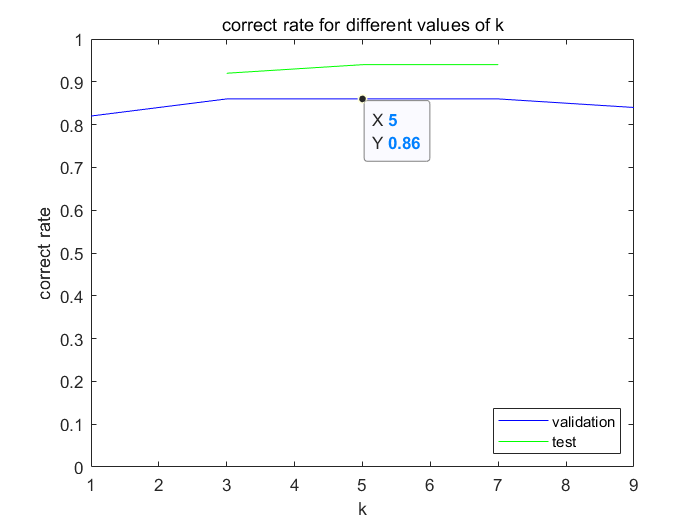
\includegraphics[scale=0.65]{figure1}
	\caption{correct rate for different values of k on validation set (blue line) and k*-2, k*, k*+2 on test set (green line)}
	\label{fig1}
\end{figure}

Then the performance of $k^*$ and $k^*\pm2$ are plot on the same figure in green. We can infer from \ref{fig1} that the test performance for these values are good enough, even higher that validation performance and the differences of correct rate btween $k^*$ and $k^*\pm2$ are small. So they correspond to the validation performance.
  
\subsection{Logistic regression}
Fistly, I write a function implementing logistic regression without regularization term (see codes in file $logistic.m$) in order to choose the best hyperparameters for the learning rate, the number of iterations, and the way in which
the weights are initialized.\par
In the function the last element of weights corresponds to bias $b$, and a column filled with $1$ is put on the right of the $data$ matrix. Now we can replace $\bm{w^Tx^{i}+b}$ with $data\times{weights}$, where $data$ and $weights$ are perspectively a $N\times(M+1)$ matrix and a $(M+1)\times1$ vector.\par
Then, we check the gradient that the function produces (see codes in file $logistic\_regression.m$). The results are as follows:

\begin{commandline}
	\begin{verbatim}
-3.4545   -3.4545
-3.5025   -3.5025
-2.6651   -2.6651
-2.7469   -2.7469
1.0465    1.0465
-3.2709   -3.2709
-2.9444   -2.9444
-9.0068   -9.0068
-0.7756   -0.7756
1.1543    1.1543
-12.5267  -12.5267

diff =

7.4413e-09
	\end{verbatim}
\end{commandline}

The gradient produced by my function corresponds to that of numerical calculation.

\begin{warn}[Notice:]
	There is a mistake in provided file $logistic\_regression\_template.m$ when calling the function $checkgrad$. Input $targets$ should be a vector filled with random integers $0$ and $1$ instead of random numbers of $U(0,1)$, so it has been modified. Besides, there is no need to pass in the argument $hyperparameters$, so it has been omitted temporarily.
\end{warn}

Next, we experiment with different hyperparameters
for the learning rate, the number of iterations, and the way weights are initialized (see codes in file $logistic\_regression.m$).\\

\paragraph{Learning rate}
Firstly, two functions $evaluate.m$ and $logistic_predict.m$ are finished. Then I fix regularizer $\lambda=0$, $number\_iterations = 100$ and initial weights $\bm{w=0}$, and change $lg(learning\_rate)$ from $-4$ to $0$, step by $0.5$. Numeric results are printed out in the command line, wchich can be seen when running the matlab code. Visualized images are displayed in \textbf{Figure \ref{fig2}, \ref{fig3}} (training set) and \textbf{Figure \ref{fig4}, \ref{fig5}} (small training set):\\

We can see from \textbf{Figure \ref{fig2}, \ref{fig3}} that cross-entropy convegences slowly with a small learning rate (e.g. $lr=10^{-4}$) and vibrates drastically with a large learning rate(e.g. $lr=10^{0}$). In the case of a small training set (\textbf{Figure \ref{fig4}, \ref{fig5}}), the models perform badly in all the learning rate, for the reason the training set is so small that has a terrible capability of generalization. So in the next 2 parts I'll only run codes on the bigger training set.\\

There is another interesting phenomenon: after the first iteration, the fraction of correct prediction rise suddenly, including models with small learning rate. This is related to the way weights are initialized. Here we fix the inital weight as $0$, which means that all the probabilities are $0.5$, exactly on the boundry of class $0$ and class $1$. That is to say, although we classify all the data as class $1$ initally, a very slight bias produced by the first iteration from the inital value of weights could change the result of the predictions to the correct direction markedly. But weights in models with small learning rate only changed slightly, so their cross-entropy are high, which means that these models predict the correct label but they are not sure enough about their predictions.\\

So, finally I choose the learning rate $10^{-1}$, whose cross-entropy is smooth and convergences qiuckly enough. And in the next parts, the learning rate will be fixed as $10^{-1}$.

\begin{figure}[H]
	\centering
	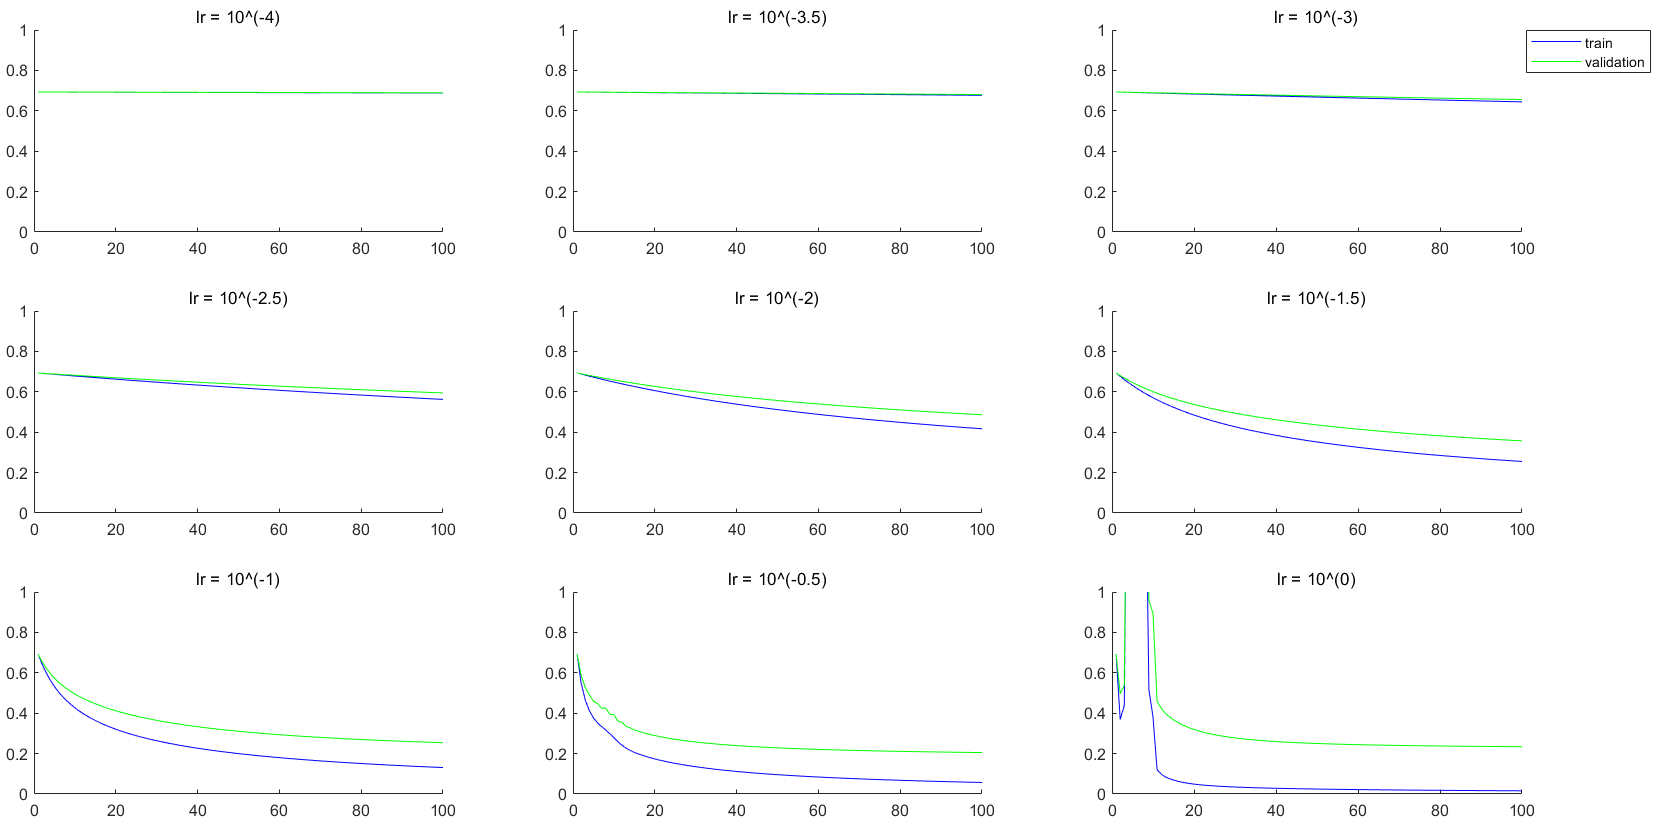
\includegraphics[scale=0.4]{figure2}
	\caption{Cross-entropy of different learning rate on training set and validation set.}
	\label{fig2}
\end{figure}

\begin{figure}[H]
	\centering
	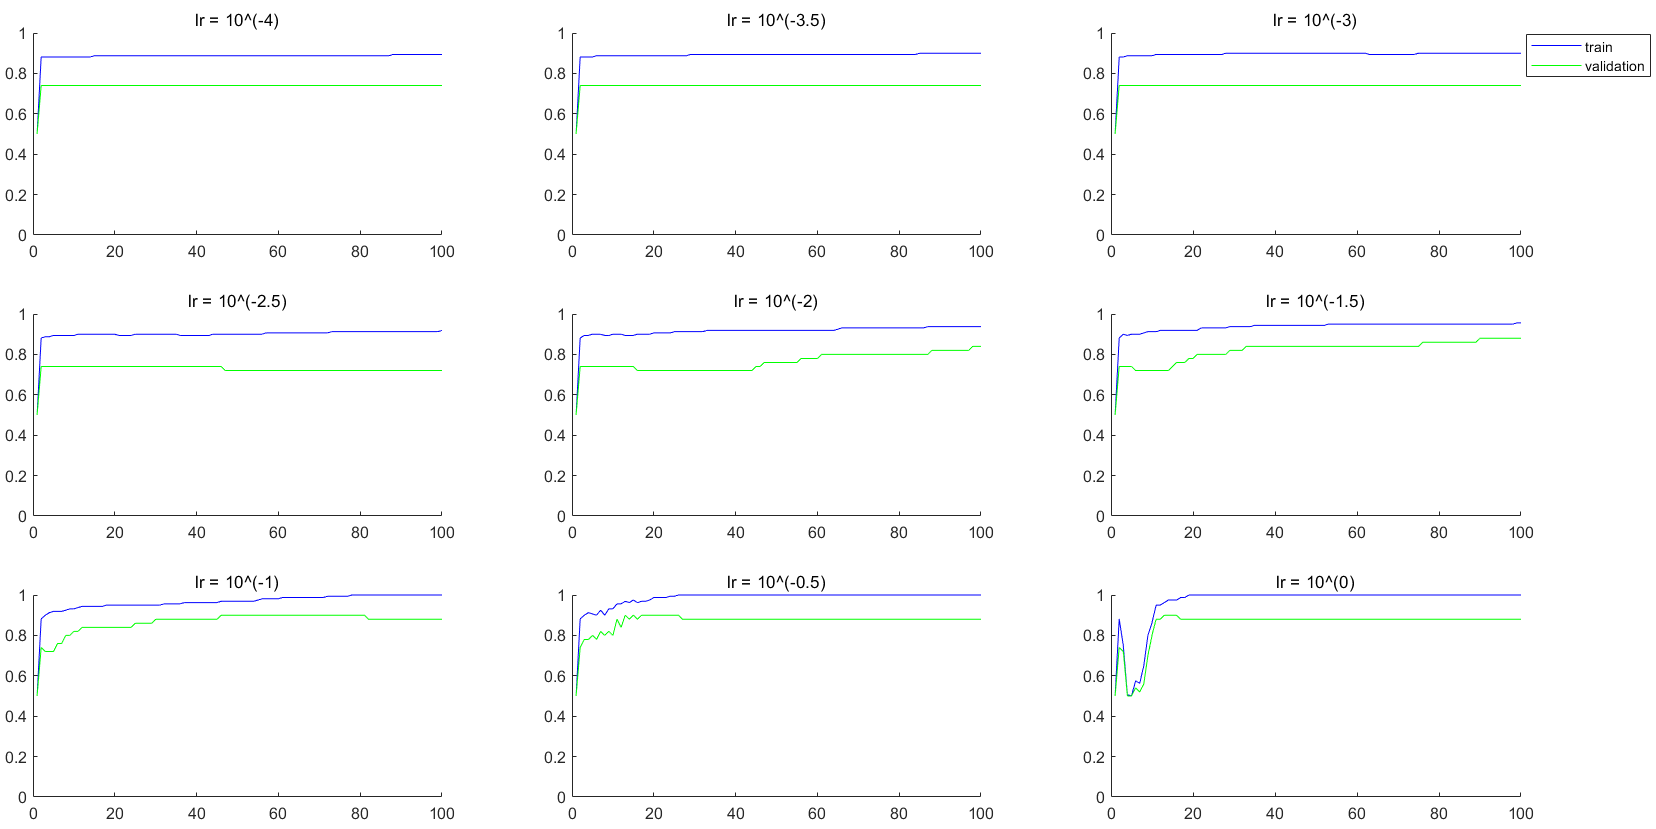
\includegraphics[scale=0.4]{figure3}
	\caption{Fraction of correct predictions for different  learning rate on training set and validation set.}
	\label{fig3}
\end{figure}

\begin{figure}[H]
	\centering
	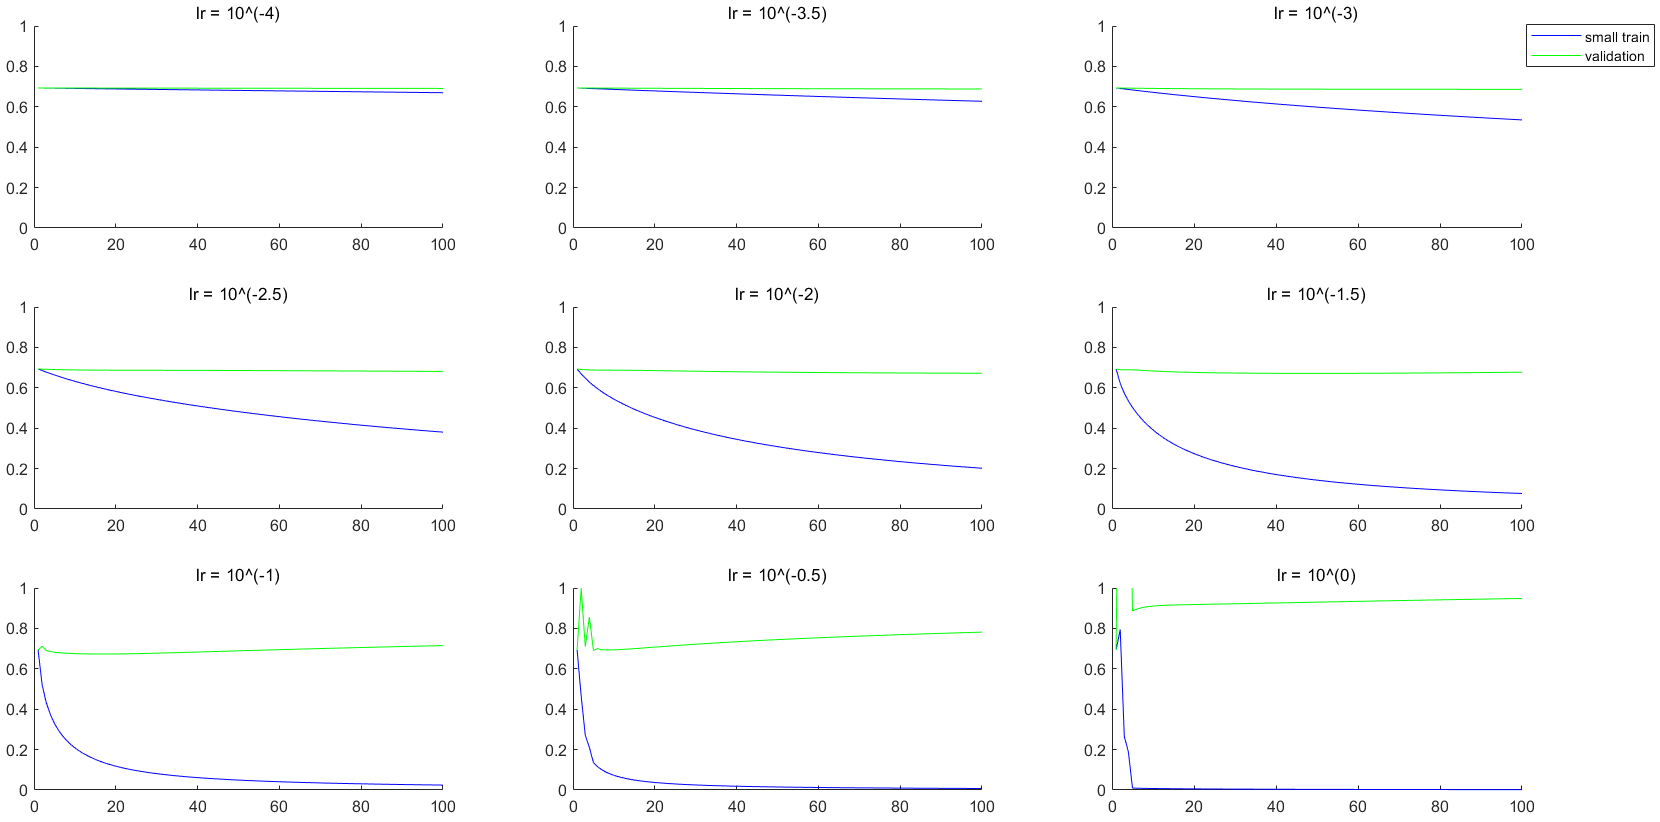
\includegraphics[scale=0.4]{figure4}
	\caption{Cross-entropy of different learning rate on small training set and validation set.}
	\label{fig4}
\end{figure}

\begin{figure}[H]
	\centering
	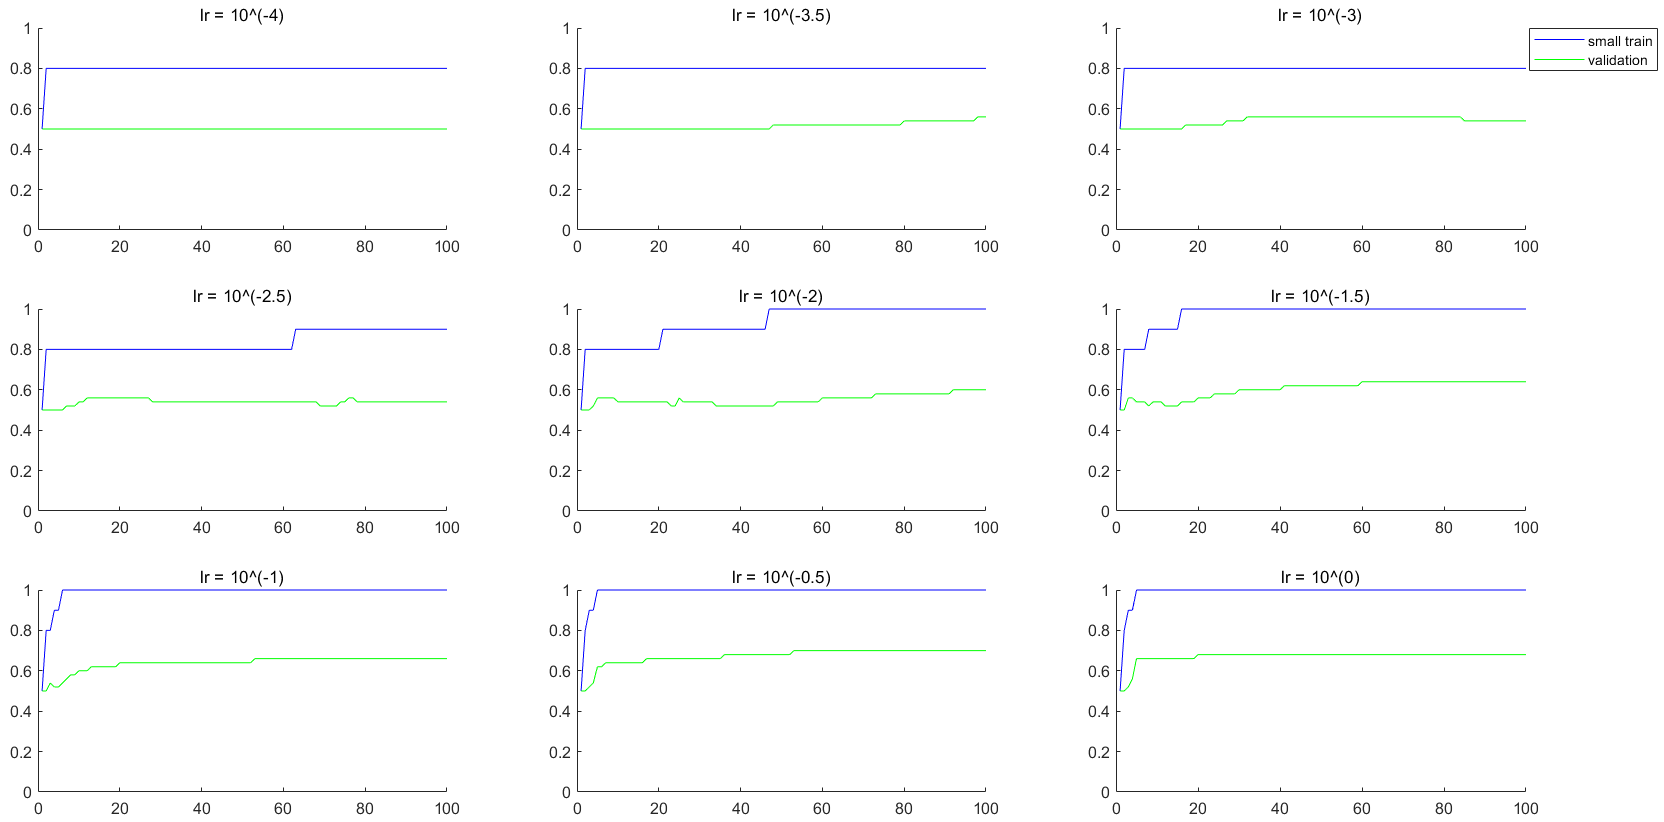
\includegraphics[scale=0.4]{figure5}
	\caption{Fraction of correct predictions for different  learning rate on small training set and validation set.}
	\label{fig5}
\end{figure}

\paragraph{Weights initialization}
In last part, we initialize the weights with all $0$, now we're going to try other kinds of initialization: uniform random numbers $U(0,1)$, Guassian random numbers $N(0,1)$ and scalar number $0, 0.5, 1$. I test these 5 kinds of approaches. Results are as follows. The curve which can't be shown represents for infinite.\\

So we choose weights all initialized with $0$ as the best approach. Just as I analysed in the part of learing rate, initializing with all $0$ can make the model on the boundary of two classes, so they can reach the right predictions easily, even with a slight iteration in the direction of its negative gradient.

\begin{figure}[H]
	\centering
	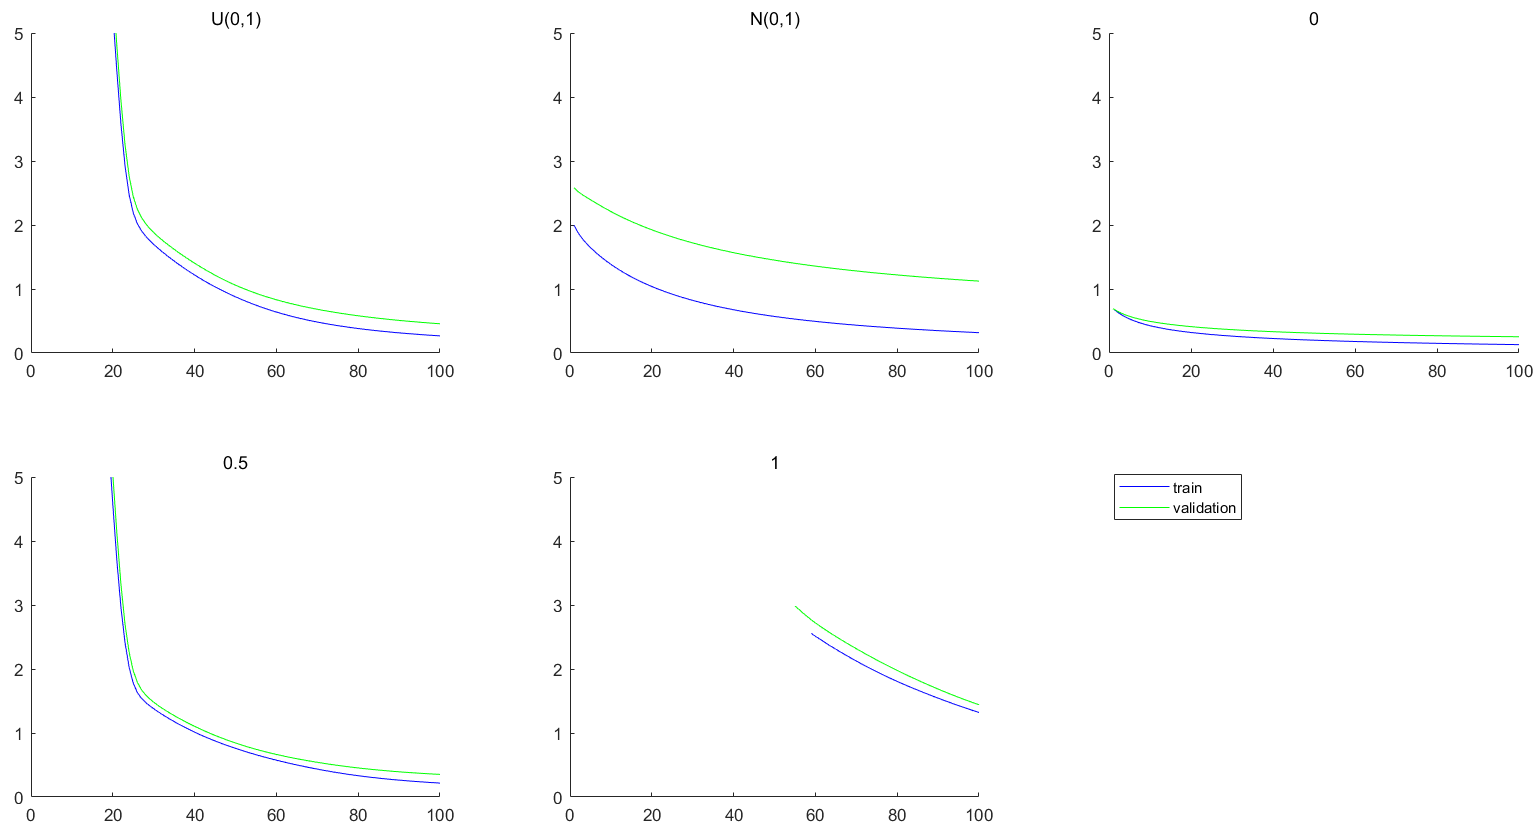
\includegraphics[scale=0.4]{figure6}
	\caption{Cross-entropy of different initial weights on training set and validation set.}
	\label{fig6}
\end{figure}

\begin{figure}[H]
	\centering
	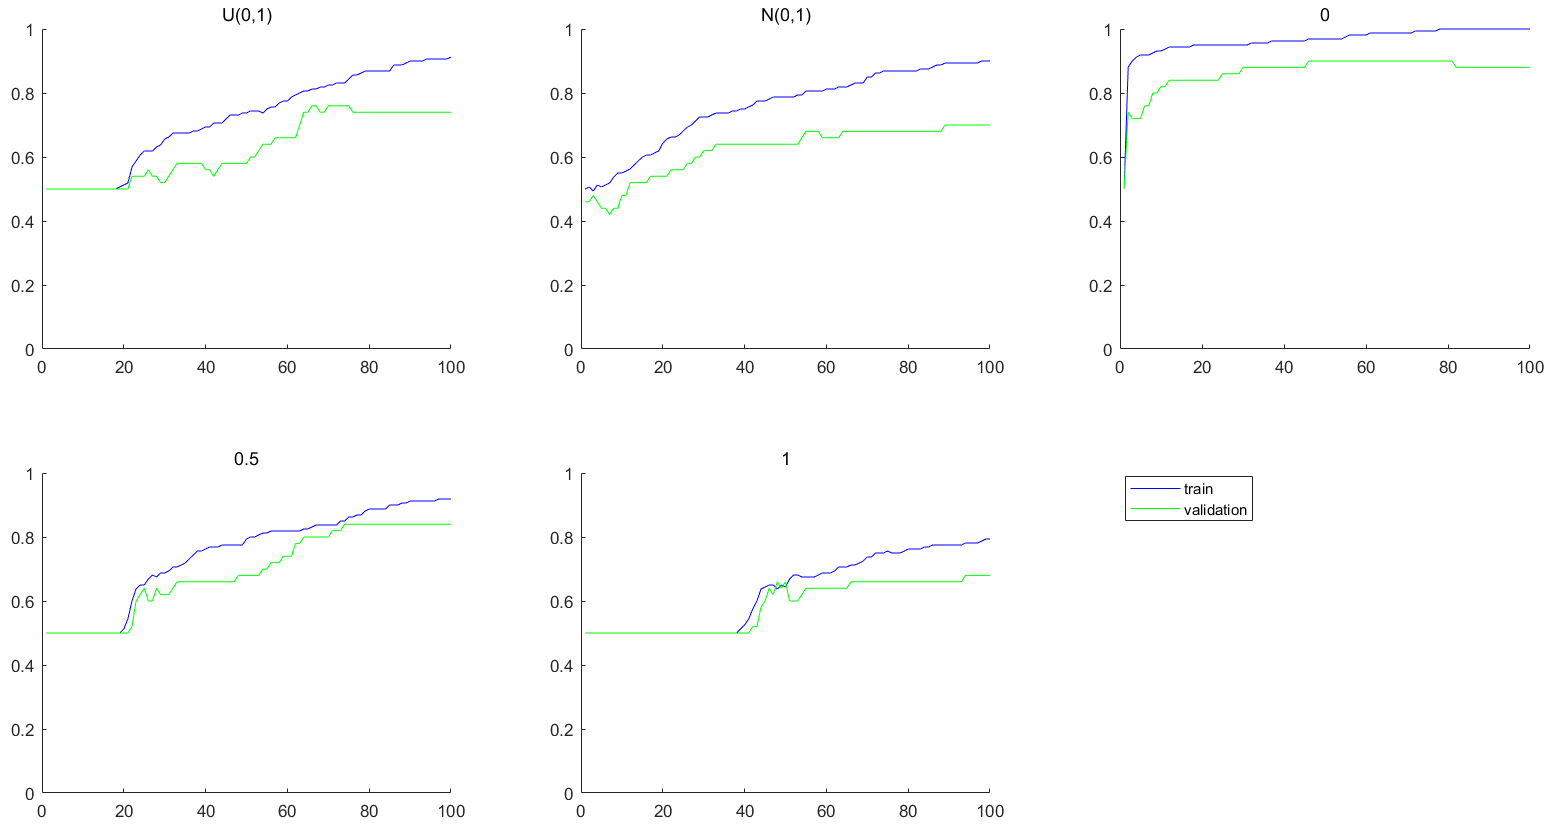
\includegraphics[scale=0.4]{figure7}
	\caption{Fraction of correct predictions different initial weights on training set and validation set.}
	\label{fig7}
\end{figure}

\paragraph{Times of iteration}
From figures above we know that the $100$ times of iteration is not sufficient for the cross-entropy to convergence. Now we choose the best learning rate and initial weights, and iterate for 1000 times, to see how many times of iteration are needed for approximate convergency of cross-entropy.\\

From \textbf{Figure \ref{fig8}} we known that cross-entropy convergences after 400 times of iteration approximately, while fraction of correct prediction convergences after 100 times of iteration approximately. In order to keep our cross-entropy loss low, we choose 400 times of iteration (for the smaller training set we only need 20 times). 

\begin{figure}[H]
	\centering
	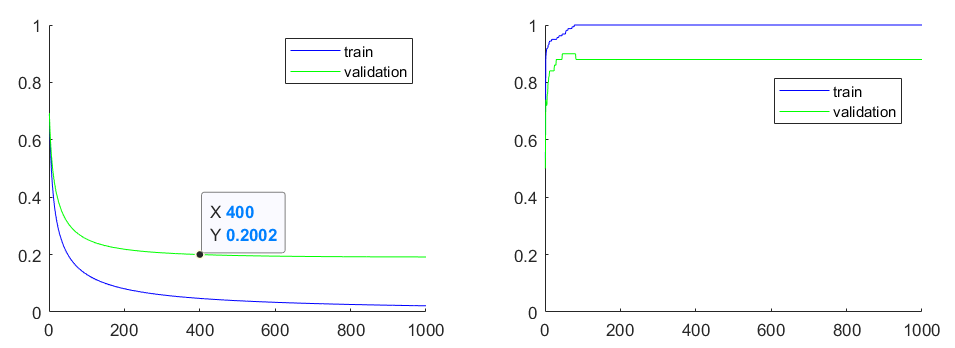
\includegraphics[scale=0.65]{figure8}
	\caption{Cross-entropy and fraction of correct predictions of different iteration times on training set and validation set.}
	\label{fig8}
\end{figure}

Finally, we choose hyperparameter settings which work the best, i.e. learining rate=0.1, inital weights=0 and iteration times= 400 (20 for the smaller training set). The results didn't change when the codes are run several times, since the model are initialized with the same weights. Results will change only when initialized with random numbers, and in this case we can compute its average cross-entropy and classification error over several times re-run.\\

We can see from the results below that the model perform well with a big training set and badly with a small one. A small training set lacking of randomness and diversity would result in a terribel capability of generalization, and needs less times of iteration to convergence.

\begin{commandline}
	\begin{verbatim}
	On minist_train:
	Train: cross-entropy 0.047368, error:0.00
	Validation: cross-entropy 0.200113, error:0.12
	Test: cross-entropy 0.201431, error:0.08
	On minist_train_small:
	Train: cross-entropy 0.117962, error:0.00
	Validation: cross-entropy 0.673644, error:0.36
	Test: cross-entropy 0.541551, error:0.24
	\end{verbatim}
\end{commandline}

\begin{figure}[H]
	\centering
	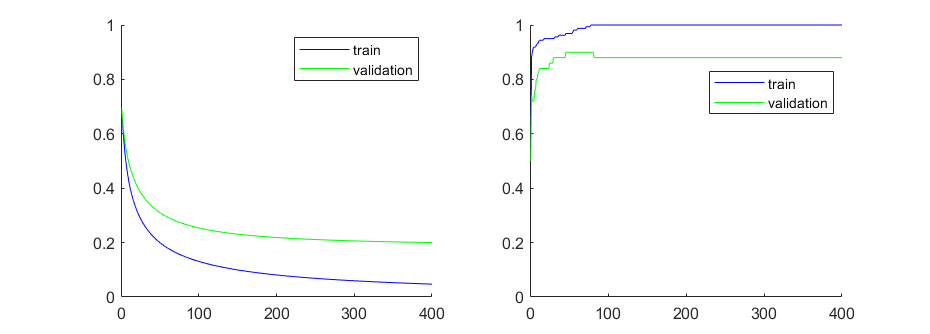
\includegraphics[scale=0.7]{figure9}
	\caption{Cross-entropy change when training with minist\_train.}
	\label{fig9}
\end{figure}

\begin{figure}[H]
	\centering
	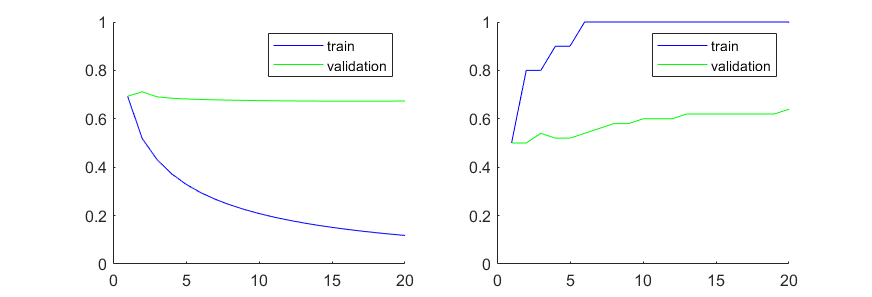
\includegraphics[scale=0.75]{figure10}
	\caption{Cross-entropy change when training with minist\_train\_small.}
	\label{fig10}
\end{figure}


\subsection{Penalized logistic regression}

To start with, function $logistic\_pen.m$ which includes a regularizer are complemented and gredients are checked. Codes in next parts are included in file $logistic\_regression\_pen.m$\par

\begin{commandline}
	\begin{verbatim}
	-4.4661   -4.4661
	1.2173    1.2173
	-2.1561   -2.1561
	-0.8216   -0.8216
	-8.5608   -8.5608
	-6.6555   -6.6555
	-3.0109   -3.0109
	-0.1498   -0.1498
	2.6396    2.6396
	3.3174    3.3174
	-2.2215   -2.2215

	diff =

	1.9515e-08
	\end{verbatim}
\end{commandline}

In order to add some randomness, here we use inital weights from $N(0,0.01)$ instead of all $0$. Re-run 50 times for each value of lambda with the weights randomly initialized each time, we get \textbf{Figure \ref{fig11}, \ref{fig12}} below. When $\lambda$ increases, the average cross entropy and classification error ($=1-fc$) go down first and then up. I think this is because $\lambda$ is related to the prior distrbution of $\bm{w}$ and $b$ ($\frac{1}{\lambda}$ is their variance). The average cross entropy and classification error will go down when $\lambda$ gets close to its real value and go up when deviate from it. So, we choose $\lambda=0.01$ ($0.1$ for the smaller training set).

\begin{figure}[H]
	\centering
	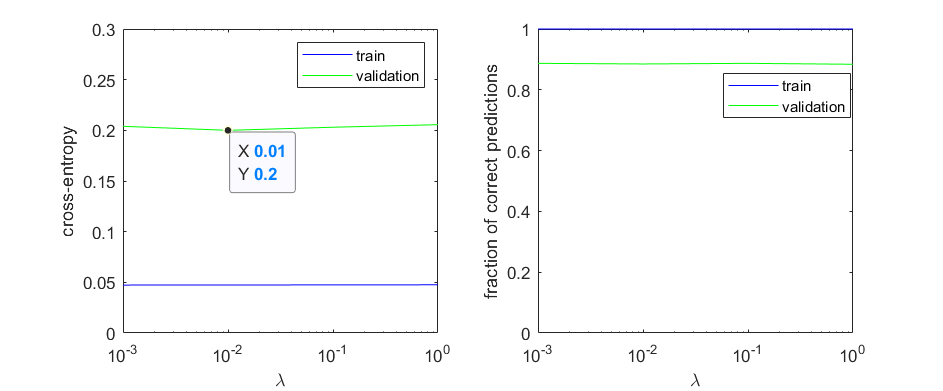
\includegraphics[scale=0.5]{figure11}
	\caption{Cross-entropy (left) and fraction of correct predictions (right) when increase $\lambda$.}
	\label{fig11}
\end{figure}

\begin{figure}[H]
	\centering
	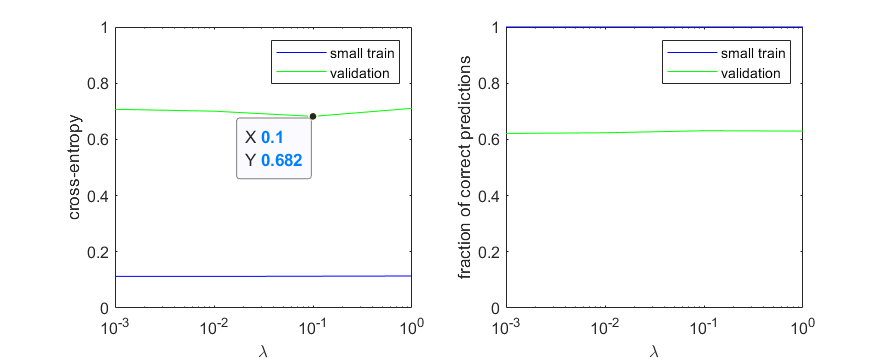
\includegraphics[scale=0.55]{figure12}
	\caption{Cross-entropy (left) and fraction of correct predictions (right) when increase $\lambda$ on smaller training set.}
	\label{fig12}
\end{figure}

Choose $\lambda=0.01$ ($0.1$ for smaller training set), the changes of cross entropy and classification error are shown in \textbf{Figure \ref{fig13}, \ref{fig14}}.\\

After including a regularizer, test errors haven't changed on both training set compared with the results in \textbf{2.2}, but cross-entropies have increased a little. It illustrates that the prior distribution only has a little influence on the model, i.e. the regularization term is relatively small compared with $E(\bm{w},b)$. But I'm convinced that the model including a regularizer would perform a bit well than the model without one in general, because it punishes weights who are so big that would influence the model heavily.\\

And obviously, the model based on the bigger training set far outweighs the model based on the smaller one. The reason has already been analysed in previous parts.

\begin{commandline}
	\begin{verbatim}
	On minist_train:
	test error = 0.0800, cross-entropy = 0.2202
	On minist_train_small:
	test error = 0.2400, cross-entropy = 0.5498
	\end{verbatim}
\end{commandline}

\begin{figure}[H]
	\centering
	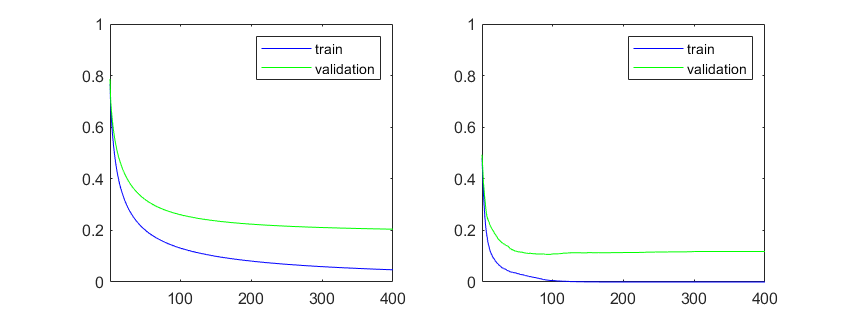
\includegraphics[scale=0.7]{figure13}
	\caption{Average cross-entropy (left) and classification error (right) when training on the bigger training set.}
	\label{fig13}
\end{figure}

\begin{figure}[H]
	\centering
	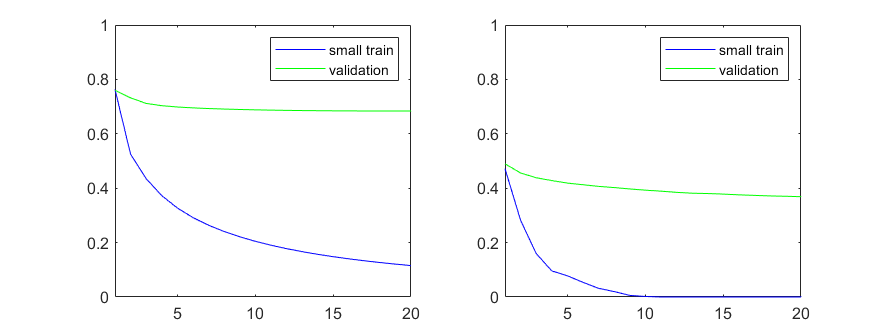
\includegraphics[scale=0.7]{figure14}
	\caption{Average cross-entropy (left) and classification error (right) when training on the smaller training set.}
	\label{fig14}
\end{figure}

\subsection{Naive Bayes}

Training and test accuracy using the naive Bayes model:
\begin{commandline}
	\begin{verbatim}
	training accuracy 0.8625
	test accuracy 0.8000
	\end{verbatim}
\end{commandline}

Visualization of the mean and variance vectors $\mu_c$ and $\sigma_c^2$ for both classes, class $0$ (hand-written number 4) is put on the top and class $1$ (hand-written number 9) on the bottom:

\begin{figure}[H]
	\centering
	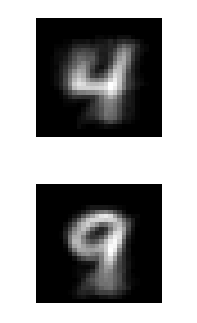
\includegraphics[scale=0.7]{figure15}
	\caption{Visualization of the mean vectors $\mu_c$.}
	\label{fig15}
\end{figure}

\begin{figure}[H]
	\centering
	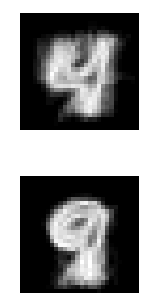
\includegraphics[scale=0.7]{figure16}
	\caption{Visualization of the variance vectors $\sigma_c^2$.}
	\label{fig16}
\end{figure}

The image of mean vectors shows the mean and approximate shape of the data, while variance implies the changing frequency of the images, where low frequency represents for the inner region of images and high frequency represents for the outline and margin of images.

\subsection{Compare k-NN, Logistic Regression, and Naive Bayes}

By the means of kNN, logistic regression and naive Bayes, the test error are respectively $6\%, 8\% \text{ and } 20\%$. The first two means perform well on this classification, while naive Bayes only have a prediciton accuracy of $80\%$.\\

kNN computes the L2 distance between each pair of our training data and test data, then vote for the correct class. Every time here comes a new set of test data, distance between each pair should be computed again. So it takes a lot of time when predicting. But it only has one hyperparameter, making it easy to asjust.

Unlike kNN, logistic regression is a parametric method. Once all the parameters have been confirmed by training, it only takes a little time to compute the possibility of each class for test data. But there are so much hyperparameters in this method that needs to be confirmed with experiment, and these hyperparameters have a big effect on the accuracy of the model. Beside, sufficient training data are required in this method in order to get a high accuracy.

As for naive Bayes, it has the easiest process of training and prediction, but often leads to a naive model with a relative low 
accuracy. This is because it has very strong assumptions that the possibility density function of every class is a normal ditribution and every class has its own covariance matrix $\sum_k$, which is diagnal (i.e. assume that every dimension of $x$ is independent). So it may perform badly when one of the assupmtions cannot be satisfied.

Furthermore, kNN has a nonlinear decision boundary, while logistic regression has a linear one and naive Bayes has a quadratic one. So their performance are affected by the distribution of each class.

\section{Stochastic Subgradient Methods}
\subsection{Averaging and Step-size Strategies}
See modified codes in matlab file $svmAvg.m$ and $run\_svm.m$.\\

Firstly, I ran the provided code $example\_svm.m$ which implements SGD. The change of objective function with training process and the final training and validation accuracy are shown below for the convenience of comparision. We can see in \textbf{Figure \ref{fig17}} that objective function never gets lower than its inital value.

\begin{figure}[H]
	\centering
	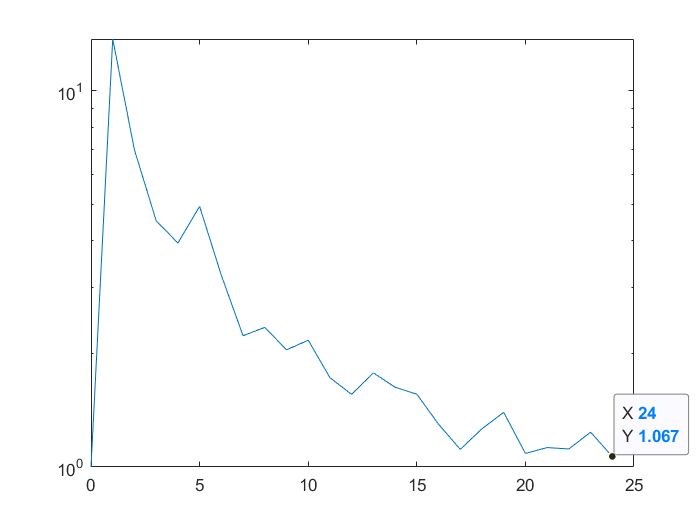
\includegraphics[scale=0.5]{figure17}
	\caption{Performance of objective function with SGD.}
	\label{fig17}
\end{figure}

\begin{commandline}
	\begin{verbatim}
	training accuracy 0.6335
	validation accuracy 0.6346
	\end{verbatim}
\end{commandline}

\paragraph{1}
In order to use running average to update the weights matrix, we use a matrix to store the gradients for all the input data. And in each loop, we update a random column (select a random $i\in\{1,2,\dots,n\}$) of our gradient table and use the average gradient to update the weights matrix. i.e.
\[
w^{t+1}=w^t-\frac{\alpha_t}{n}\sum_{i=1}^{n}g_i^{t+1}-\alpha_t\lambda w^t ,\text{ where } g_i^{t+1}=
\begin{cases}
\nabla f(w^t)& \text{i=i(t)}\\
g_i^t& \text{otherwise}
\end{cases}
\]

Critical codes are shown below, where $gt$ is the matrix storing the all the gradients and sg is computed sub-gradient.

\begin{lstlisting}
    % Updata the gradient table and its mean
	gt_sum = gt_sum - gt(:,i) + sg;
	gt(:,i) = sg;
	
	% Take SAG step
	w = w - alpha * (gt_sum / n + lambda*w);
\end{lstlisting}

Corresponding results are as shown in \textbf{Figure \ref{fig18}}, and training and validation accuracy are also presented. We can see that the objective function goes extremely high in the beginning of the iterations, while few gradients are updated during this period. So the objective function just went along the wrong direction and increased quickly. After sufficient iterations, most of the gradients are updated, so their average is approximately the correct direction of gradient, leading the objective function going down. But finally objective function gets lower than its initial value, with training and validation accuracy a little higher than that of SGD, which means we get a slightly better results than SGD.

\begin{figure}[H]
	\centering
	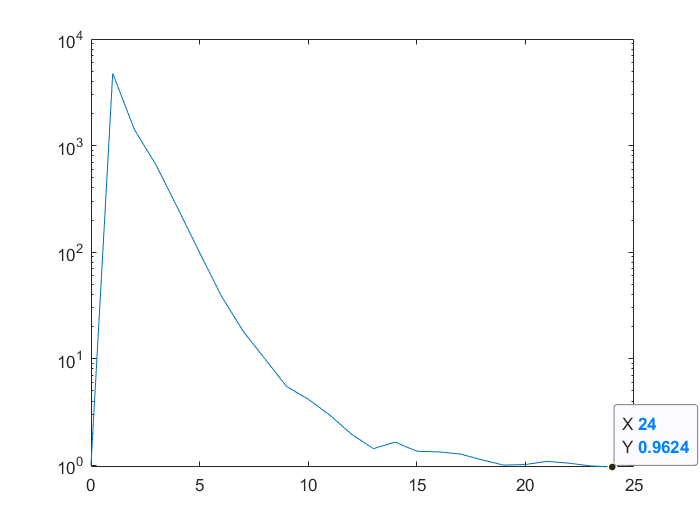
\includegraphics[scale=0.5]{figure18}
	\caption{Performance of objective function with averaging.}
	\label{fig18}
\end{figure}

\begin{commandline}
	\begin{verbatim}
	training accuracy 0.6651
	validation accuracy 0.6590
	\end{verbatim}
\end{commandline}

\paragraph{2}

To solve the problem occurred in the last part, we use SGD in the first half iterations and SAG the rest, making sure that most of gradients in the gradient table had been updated.\\

Critical codes are presented below.

\begin{lstlisting}
	% Take SAG step
	if t < maxIter/2
	w = w - alpha * (sg + lambda*w);
	else
	w = w - alpha * (gt_sum / n + lambda*w);
	end
\end{lstlisting}

In \textbf{Figure \ref{fig19}}, we can see clearly that the first half of iterations have the same shape as the SGD, and the second half reaches a point lower than the inital value, which is the same as SAG. Besides, training and validaiton accuracy are about the same as SAG.

\begin{figure}[H]
	\centering
	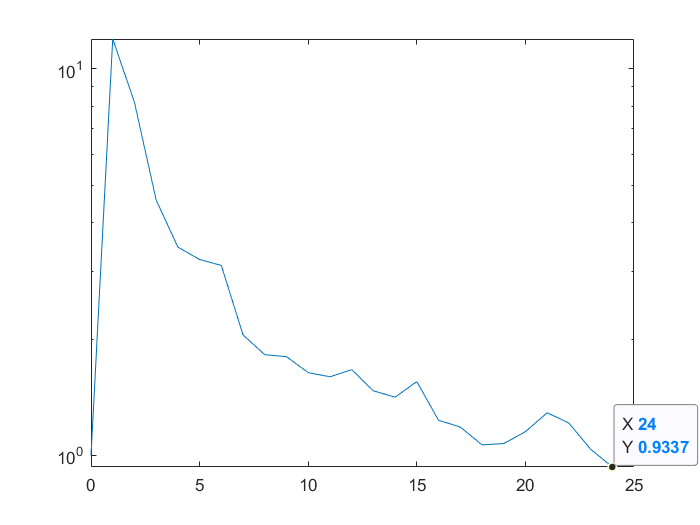
\includegraphics[scale=0.5]{figure19}
	\caption{Performance of objective function with "second-half" averaging.}
	\label{fig19}
\end{figure}

\begin{commandline}
	\begin{verbatim}
	training accuracy 0.6572
	validation accuracy 0.6563
	\end{verbatim}
\end{commandline}

\paragraph{3}

So as to optimize its performance, I tried to adjust some of the hyperparameters such as regularization parameter $\lambda$, learning rate $\alpha_t$ and the proportion of SGD and SAG. I found it most effective to zoom in the $\lambda$ 1000 times, and it take about $5\times{n}$ iterations to convergence instead of $25\times{n}$ iterations (Show in \textbf{Figure \ref{fig20}}). And finally reaches a validation accuracy of 70.56\%, much higher than initial SGD.\

This is easy to interpret: objective function changed intensely in \textbf{Figure \ref{fig17} ,\ref{fig18} ,\ref{fig19}}, which implies that the weights changed violently, maybe some too big and some too small. Strengthen the L2 regularization could help restrain the fast increasing of weights, keeping all of them not so big. Therefore, the objective function could convengerce more quickly.

\begin{figure}[H]
	\centering
	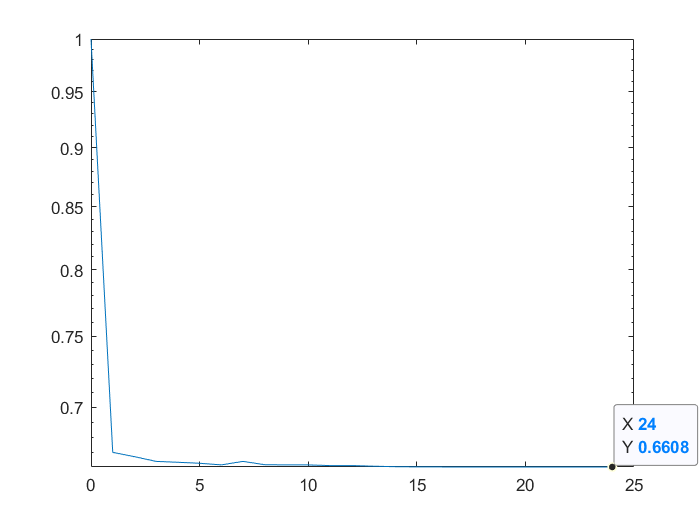
\includegraphics[scale=0.5]{figure20}
	\caption{Performance of objective function with $\lambda$ magnified to 1000 times.}
	\label{fig20}
\end{figure}

\begin{commandline}
	\begin{verbatim}
	training accuracy 0.7100
	validation accuracy 0.7056
	\end{verbatim}
\end{commandline}


%----------------------------------------------------------------------------------------

\end{document}
